Ein Skifahrer mit der Masse \mO\ (mit Ausrüstung) gleitet in Falllinie eine Piste hinunter, die pro \lPO\ entlang des Hangs um \hPO\ an Höhe verliert. Die Reibungszahl zwischen Ski und Schnee beträgt \muGO; der Luftwiderstand ist vernachlässigbar. Rechne mit \gO.

\begin{center}
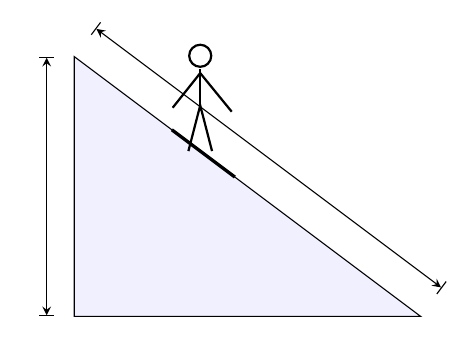
\begin{tikzpicture}[>=stealth]
 \draw[fill=blue!6] (0,3.3) -- (4.4,0) -- (0,0) -- cycle;
 \draw[very thick] (1.24,2.37) -- (2.04,1.77);
 \draw[thick] (1.45,2.1) -- (1.6,2.68) -- (1.75,2.1);
 \draw[thick] (1.6,2.68) -- (1.6,3.14);
 \draw[thick, fill=white] (1.6,3.31) circle (0.14);
 \draw[thick] (1.6,3.09) -- (1.25,2.65);
 \draw[thick] (1.6,3.09) -- (2,2.6);
 \draw[|<->|, thin] (0.27,3.66) -- node[above right] {\lPO} (4.67,0.36);
 \draw[|<->|, thin] (-0.35,0) -- node[left] {\hPO} (-0.35,3.3);
\end{tikzpicture}
\end{center}

\begin{abcliste}
\abc
Wie gross ist die Normalkraft?

\abc
Mit welcher Beschleunigung wird der Skifahrer schneller?
\end{abcliste}
